% Chapter 3 from the thesis template file
%   that contains an example table and figure.
\chapter{METHODS AND PROCEDURES}

\section{Capacitive Skin Sensor}
The strain sensor used in this project is a soft elastomeric capacitor (SEC) developed by the Department of Civil, Construction, and Environmental Engineering at Iowa State University.  The SEC is composed of a nanocomposite mix of poly-styrene-co-ethylene-co-butylene-co-styrene (SEBS) (Dryfelx 500120) doped with rutile $TiO_2$ (Sachtleben R 320 D) serving as a dielectric for the capacitor\cite{soft-elastomeric-capacitor}.

\subsection{Capacitive properties}
The strain to capacitance properties were shown by Dr. Laflamme et al. to be the form shown in Equation \ref{cap-prop-eq1}.  The parameter $C_0$ is the nominal capacitance of the sensor and is estimated to be in the range of 500pF.  The value of the gain factor $\lambda$ is dependent on the geometry of the sensor; it is 2 for the capacitive skin sensors used in this study.  The value of $\epsilon_s$ is the strain seen by the sensor and $\Delta C$ is the change in the capacitance of the sensor due to that strain.  This can be rewritten in the form of Equation \ref{cap-prop-eq2}

\begin{eqnarray}
	\frac{\Delta C}{C_0}&=&\lambda \epsilon_s\label{cap-prop-eq1}\\
	\Delta C &=& \lambda C_0 \epsilon_s\label{cap-prop-eq2}
\end{eqnarray}

The overall capacitance of the strain sensor is the nominal capacitance plus the capacitance due to an applied strain.  This capacitance $C_{sens}$ is shown in Equation \ref{cap-prop-eq3}.  The capacitance due to strain is much smaller than the nominal capacitance; it is on the order of femtofarads for an applied strain of one micro strain.  The typical values for the parameters of a capacitive skin sensor are shown in Table \ref{cap-strain-table}.

\begin{equation}
	C_{sens}=C_0+\Delta C=C_0+\lambda C_0\epsilon_s=C_0(1+\lambda\epsilon_s)\label{cap-prop-eq3}
\end{equation}

\begin{table}\centering
	\begin{tabular}{|l|l|}
		\hline
		Parameter & Typical Value\\
		\hline
		$C_0$ & 500pF\\
		$\lambda$ & 2\\
		\hline
	\end{tabular}
	\caption{Typical capacitive strain gauge parameters}\label{cap-strain-table}
\end{table}

\section{Capacitive Measurement Circuit}
\subsection{Challenges}
The capacitance change that needed to be measured was on the order of $1fF$ on a capacitor with a nominal capacitance of $500pF$.  This is a change on the order of one part per 500,000.  Using traditional methods of capacitance measurement is unable to measure at this required sensitivity.  

\subsubsection{Traditional Methods of Capacitance Measurement}
There are many traditional methods for measuring capacitance which were explored as possible solutions and determined to be ineffective for solving this problem.  To accurately measure these small changes in capacitance a circuit with a high sensitivity to capacitance change is required.  Sensitivity is the measure of how much a output parameter changes due to a change of an input parameter.  In general the equation for sensitivity is given in Equation \ref{sens-eq1} where $x$ is the input parameter and $y$ is the output parameter.

\begin{equation}
	S=\lim_{\Delta x\rightarrow0}\frac{\Delta y/y}{\Delta x/x}=\frac{x}{y}\frac{\partial y}{\partial x}\label{sens-eq1}
	%\caption{General sensitivity equation}
\end{equation}

In the context of measuring the capacitance of the stain sensor where the base capacitance is $C_0$ and the change in capacitance is $\Delta C$ define the output parameter as the frequency at capacitance $C$ is define as $f(C)$, then the sensitivity equation becomes the form shown in Equation \ref{sens-eq2} or Equation \ref{sens-eq3}.

\begin{eqnarray}
	S&=&\lim_{\Delta C\rightarrow 0}\frac{\left(f\left(C_0+\Delta C\right)-f\left(C_0\right)\right)C_0}{ f(C_0)\Delta C}\label{sens-eq2}\\
	&=&\frac{C_0}{f(C_0)}\left[\frac{\partial f(C)}{\partial C}\right]_{C=C_0}\label{sens-eq3}
\end{eqnarray} 

\paragraph{LCR oscillator circuits} 
are circuits that oscillate at a frequency proportional to the capacitance of the sensor and fixed inductor value.  The frequency of these circuits is proportional to $1/\sqrt{C}$.  Given the sensitivity equation in Equation \ref{sens-eq3} the sensitivity of a LCR oscillator circuit can be calculated in Equation \ref{sens-lcr}.

\begin{eqnarray}
	f&:=&\frac{\alpha}{\sqrt{(C)}}\\
	S&=&\frac{C_0\sqrt{C_0}}{\alpha}\left[\frac{-\alpha}{2C\sqrt{C}}\right]_{C=C_0}=-1/2\label{sens-lcr}
\end{eqnarray} 

Therefore this circuit has a very small sensitivity to changes in capacitance is not a valid solution for the problem.

\paragraph{Charge time measurement} 
is a method of measuring the capacitance of a circuit by measuring the time for that circuit to charge to a set amount.  This method involves charging the capacitor with a constant current source and measuring the time to charge to one time constant.  The voltage through a capacitor which is charging by a constant current source $I$ is $V(t)=\frac{I}{C}t$.  Therefore if the measured parameter is the time $t$ to charge to a given voltage $V$ the time to charge is given in Equation \ref{sens-ctm-eq1}, then from Equation \ref{sens-eq1} the sensitivity is given in Equation \ref{sens-ctm-eq2}

\begin{equation}
	t=\frac{C}{I}V\label{sens-ctm-eq1}
\end{equation}

\begin{equation}
	S=\frac{C_0}{C_0V/I}\frac{V}{I}=1\label{sens-ctm-eq2}
\end{equation}

\paragraph{A relaxation oscillator} 
is a simple type of oscillator which produces a square wave at a frequency proportional to the capacitor value.  The circuit for a basic relaxation oscillator is shown in Figure \ref{simp-relax-osc}.  This circuit oscillates at a frequency $f$ show in Equation \ref{sens-relax-eq1}.

\begin{equation}
	f=\frac{1}{2\ln(3)RC}\label{sens-relax-eq1}
\end{equation} 

Therefor the sensitivity can be calculated using Equation \ref{sens-eq3} and is shown in Equation \ref{sens-relax-eq2}.

\begin{equation}
	S=\frac{C_0}{1/(2\ln(3)RC_0)}\frac{-1}{2\ln(3)RC_0^2}=-1\label{sens-relax-eq2}
\end{equation}

\begin{figure}
	\begin{center}
		
\includegraphics[width=.6\textwidth]{Images/RelaxationOsc.png}
		\caption{Simple relaxation oscillator circuit.\label{simp-relax-osc}}
	\end{center}
\end{figure}

\subsection{Design}
None of the traditional methods of capacitance measurements explored are capable of achieving the sensitivity required to accurately measure the small changes of capacitance produced by the strain sensor.  For example, if the relaxation oscillator was used to measure a $1fF$ change in a $500pF$ capacitor assuming $R=910\Omega$ yields the frequencies shown in Equations \ref{design-eq1} and \ref{design-eq2}.

\begin{eqnarray}
	f_{\text{unstrained}}&=&\frac{1}{1820\Omega\ln(3)(500\text{pF})}=1.0002628864 \text{MHz}\label{design-eq1}\\
	f_{\text{strained}}&=&\frac{1}{1820\Omega\ln(3)(500\text{pF}+1\text{fF})}=1.00026088588 \text{MHz}\label{design-eq2}
\end{eqnarray}

This corresponds to a change in frequency of approximately 2Hz; an effective change of two parts per million.  Clearly it is impractical to measure this value in a real system.  A system had to be designed to greatly increase the sensitivity of the data acquisition circuit to the expected small changes in capacitance.

The problem with the other capacitance measurement techniques is the relatively large nominal capacitance of the skin sensor to its small change in capacitance due to an applied strain.  The approximate expected nominal capacitance is 500pF with a change of capacitance on the order of 1fF; this is a change of one part per five-hundred thousand.  The overall range of capacitance change expected is relatively small in comparison to the nominal capacitance; in the case of a sensor measuring 500 micro-strain can expect a capacitance change of 500fF or 0.5pF.  Define the variable $C_{max}$ as this maximum expected capacitance change.  The solution is therefore to cancel out the nominal capacitance such that the only capacitance contributing to the measured frequency is the capacitance due to strain.

The equivalent capacitance of capacitors in parallel is the sum of the capacitance of each capacitor.  Therefore connecting the strain sensor in parallel with a capacitor of $C$ shown in Equation \ref{design-eq3} will yield an equivalent capacitance of $C_1$.  By designing the system such that $C_1=C_{max}+\epsilon$ the capacitance over the range of $\pm500$ micro-strain will be $\epsilon\leq C_{eq} \leq C_{max}+\epsilon$.  This capacitance $C_{eq}$ can be used as an input to one of the traditional capacitance measurement techniques.

\begin{equation}
	C=C_1-C_0\label{design-eq3}
\end{equation} 

The relaxation oscillator circuit was chosen due to its higher sensitivity, relatively cheaper cost, and lower energy requirements compared to the other measurement techniques.

\subsubsection{Negative capacitive circuit}
The basic negative capacitor circuit used for this project is shown in Figure \ref{neg-fig-1}.  This is a well established and common configuration used to create negative impedance circuits.  It has many useful features including the ease of setting the impedance by changing the value of a single potentiometer.

\begin{figure}
	\begin{center}
		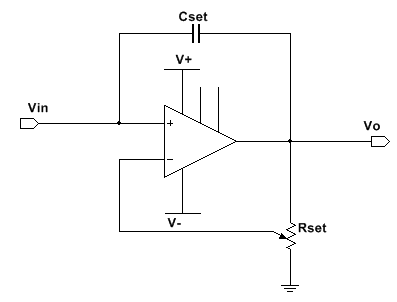
\includegraphics[width=.6\textwidth]{Images/neg-cap-circ.png}
		\caption{Negative capacitance circuit schematic\label{neg-fig-1}}
	\end{center}
\end{figure}

\paragraph{The negative feedback} circuit forms a basic voltage divider circuit between the Op-Amp output and ground.  Therefore the Op-Amp output voltage $V_o$ is given in Equation \ref{neg-eq1} where $x\in[0,1]$ is the position of the potentiometer.

\begin{equation}
	V_o=\frac{1}{x}V_{in}\geq V_{in}\label{neg-eq1}
\end{equation}

\paragraph{The positive feedback} circuit has an impedance $Z_{set}=\frac{1}{sC_{set}}$ where $s$ is the Laplace operator.  The input current $I_{in}$ can be calculated using Equation \ref{neg-eq2}.  This represents the current sunk or sourced at the input to the negative impedance circuit.

\begin{equation}
	I_{in}=\frac{V_{in}-V_o}{Z_{set}}\label{neg-eq2}
\end{equation}

\paragraph{The circuit impedance} of the negative impedance circuit is given by Ohms law as $V_{in}=ZI_{in}$.  Using the calculated $V_o$ from the negative feedback circuit and using that into the positive feedback circuit calculation the impedance of the circuit is calculated in Equation \ref{neg-eq3}.  Using the fact that $Z=\frac{1}{sC_{set}}$ the equivalent capacitance of the circuit is shown in Equation \ref{neg-eq4}.

\begin{eqnarray}
	I_{in}&=&\frac{V_{in}-\frac{1}{x}V_{in}}{Z_{set}}\\
	&=&\frac{\frac{x-1}{x}V_{in}}{Z_{set}}\\
	&\Downarrow&\nonumber\\
	Z_{eq}=\frac{V_{in}}{I_{in}}&=&\frac{x}{x-1}Z_{set}\leq0\label{neg-eq3}
\end{eqnarray}

\begin{equation}
	Z_{eq}=\frac{1}{sC_{eq}}=\frac{x}{sC_{set}(x-2)}\Rightarrow C_{eq}=\frac{x-1}{x}C_{set}\label{neg-eq4}
\end{equation}

In the implementation the potentiometer is digitally controlled to allow real time calibration of the system.  The potentiometer chosen was the CAT5259 manufactured by ON Semiconductors.  This potentiometer divides the range linearly into eight bits of resolution.  Therefore the $x$ in Equation \ref{neg-eq4} must be chosen such that $x\in\{\frac{k}{2^8}: k\in\mathbb{N}, k<2^8\}$.  Therefore the equivalent capacitance of the circuit in terms of the integer value $k\in[0,256)$ is shown in Equation \ref{neg-eq5}.

\begin{eqnarray}
	C_{eq}&=&\frac{x-1}{x}C_{set}\label{neg-eq6}\\
	\frac{C_{eq}}{C_{set}}&=&\frac{k-2^8}{k}\label{neg-eq5}
\end{eqnarray}

This capacitance is plotted over the range of $k\in[23,255]$ and $k\in[85,255]$ in Figures \ref{neg-fig1} and \ref{neg-fig2} respectively.  By choosing $C_{set}\approx C_0$ of the sensor the negative capacitor circuit can stay within the nearly linear region shown in Figure \ref{neg-fig2}.

\begin{figure}
	\begin{center}
		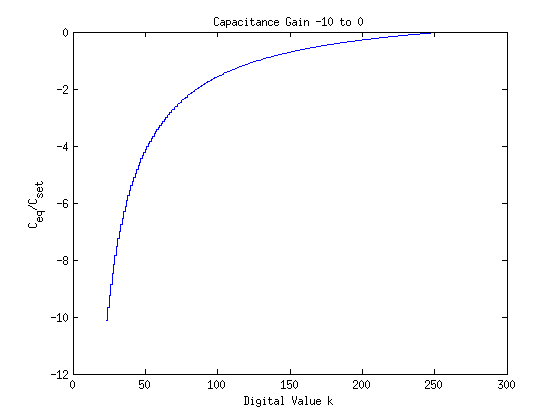
\includegraphics[width=.6\textwidth]{Images/neg-cap-gain-1.png}
		\caption{Negative capacitance gain from -10 to 0\label{neg-fig1}}
	\end{center}
\end{figure}

\begin{figure}
	\begin{center}
		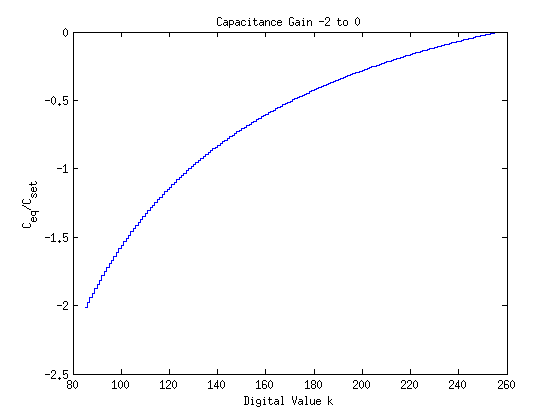
\includegraphics[width=.6\textwidth]{Images/neg-cap-gain-2.png}
		\caption{Negative capacitance gain from -2 to 0\label{neg-fig2}}
	\end{center}
\end{figure}

\subsubsection{Relaxation oscillator}
The same relaxation circuit shown in Figure \ref{simp-relax-osc} is used to convert the change in capacitance into a change in frequency with the one key change: the capacitor is the parallel combination of the sensor $C_{sens}$ and the negative capacitance $C_{1}$.  The equivalent capacitance of this parallel combination is the sum of both capacitors, $C=C_{sens}+C_1$ where $C_1$ is the equivalent capacitance of the negative capacitance circuit calculated in Equation \ref{neg-eq6}. 

Assuming all resistors $R$ in the relaxation oscillator are equal the frequency output of the oscillator is repeated in Equation \ref{relax-eq1}.  Using the new value for the capacitance input of the oscillator yields a new frequency equation shown in Equation \ref{relax-eq2}.  Combining the definition of $C_1$ from Equation \ref{neg-eq6} the equation shown in Equation \ref{relax-eq3} can be obtained for the frequency output in terms of the $C_{sens}$ and digital value $k$.

\begin{eqnarray}
	f(C)&=&\frac{1}{2\ln(3)RC}\label{relax-eq1}\\
	f(C_{sens},C_1)&=&\frac{1}{2\ln(3)R(C_{sens}+C_1)}\label{relax-eq2}\\
	f(C_{sens},k)&=&\frac{1}{2\ln(3)R(C_{sens}+\frac{k-256}{k}C_{set})}\label{relax-eq3}
\end{eqnarray}

From the model of the capacitive skin sensor, the value of $C_{sens}$ has two components: the first component is the unstrained base capacitance and the second is the change in capacitance due to strain.  Therefore by writing $C_{sens}$ in the form of Equation \ref{relax-eq4} the frequency equation in Equation \ref{relax-eq3} becomes Equation \ref{relax-eq5}.

\begin{eqnarray}
	C_{sens}&=&C_0+\Delta C\label{relax-eq4}\\
	f(\Delta C,k)&=&\frac{1}{2\ln(3)R(C_0+\frac{k-256}{k}C_{set}+\Delta C)}\label{relax-eq5}	
\end{eqnarray}

\paragraph{The sensitivity} of this new capacitive measurement system can be calculated using the definition of sensitivity given in Equation \ref{sens-eq3} and the frequency equation given in Equation \ref{relax-eq3}.  First the derivative of the frequency with respect to the capacitance of the sensor is calculated in Equation \ref{relax-eq6}.  Form this the sensitivity can be calculated in Equation \ref{relax-eq7}.  Including the definition of $C_{sens}$ given in Equation \ref{relax-eq4} gives the resulting sensitivity in Equation \ref{relax-eq8}.

\begin{eqnarray}
	\frac{\partial f(C_{sens})}{\partial C_{sens}}&=&\frac{\partial}{\partial C_{sens}}\left[\frac{1}{2\ln(3)R(C_{sens}+\frac{k-256}{k}C_{set})}\right]\\
	&=&\frac{1}{2\ln(3)R(C_{sens}+\frac{k-256}{k}C_{set})^2}\label{relax-eq6}\\
	S&=&\frac{C_{sens}}{f(C_{sens})}\frac{\partial f(C_{sens})}{\partial C_{sens}}\\
	&=&\frac{C_{sens}(2\ln(3)R(C_sens+\frac{k-256}{k}C_{set})}{2\ln(3)R(C_{sens}+\frac{k-256}{k}C_{set})^2}\\
	&=&\frac{C_{sens}}{C_{sens}+\frac{k-256}{k}C_{set}}\label{relax-eq7}\\
	&=&\frac{C_0+\Delta C}{C_0+\frac{k-256}{k}C_{set}+\Delta C}\\
	&=&\frac{C_0}{C_0+\frac{k-256}{k}C_{set}+\Delta C}+\frac{\Delta C}{C_0+\frac{k-256}{k}C_{set}+\Delta C}\label{relax-eq8}
\end{eqnarray}

Define a new variable $\alpha$ as given in Equation \ref{relax-eq9}.  By choosing $k$ and $C_{set}$ such that $\alpha$ is small the sensitivity becomes very large reaching a theoretical maximum of $C_0/\Delta C+1$ when $\alpha=0$.

\begin{eqnarray}
	\alpha&:=&C_0+\frac{k-256}{k}C_{set}\label{relax-eq9}\\
	S&=&\frac{C_0}{\alpha+\Delta C}+\frac{\Delta C}{\alpha +\Delta C}\label{relax-sens-eq}
\end{eqnarray}

\paragraph{Parameter selection} is based on the design requirements.  The design requirements specify the need to measure $1\mu\epsilon$ resolution over a range of $\pm500\mu\epsilon$ from unstrained.  Define $\Delta C_\epsilon$ to be the change in capacitance of the sensor due to a $1\mu\epsilon$ strain, then the maximum and minimum values of $\Delta C$ are $\Delta C_{max}=500\Delta C_\epsilon$ and $\Delta C_{min}=-500\Delta C_\epsilon$ respectively.

To achieve maximum sensitivity $\alpha$ must be chosen as small as possible; however, if the denominator of Equation \ref{relax-eq5} becomes negative the system poles of the system will move into the right half plan causing the circuit to become unstable.  Therefore the constrain equation shown in Equation \ref{relax-eq10} must be true for all $\Delta C$ in the range.

\begin{eqnarray}
	C_0+\frac{k-256}{k}C_{set}+\Delta C = \alpha + \Delta C &>& 0, \quad\forall\quad \Delta C\in[\Delta C_{min}, \Delta C_{max}]\label{relax-eq10}\\
	\alpha &>& -C_{min}\label{relax-eq11}
\end{eqnarray}

Using this value of $\alpha$ the values of $C_{set}$ and $k$ can be set.  Choose $C_{set}\approx 2C_0$ to force $k$ into a sensitive and approximately linear region in Figure \ref{neg-fig2}.  Since the nominal capacitance of the capacitive skin sensors is approximately 500pF choose $C_{set}=$1nF.  With this value $k$ can be calculated to be 171 giving making $\alpha=2.9\times10^{-12}$.  Plugging these numbers into Equation \ref{relax-sens-eq} gives a theoretical sensitivity of $3.4\times10^{11}$.  It should be noted that this theoretical value could never be achieved in a real system; however, this shows the high sensitivity potential of this circuit.

The capacitive sensor is characterized for oscillation frequencies under one kilohertz.  

\subsection{Output}
The output form the data acquisition circuit is a square wave which has a frequency dependent on the strain of the sensor.  The frequency of the square wave is depended on the capacitor $C_{set}$, the set potentiometer value, and the resistor value $R$ of the oscillator.  The higher this frequency is for a given value of $R$ the higher the overall sensitivity of the system; however, there is a physical limit of sampling frequency for the capacitive sensor that the frequency must remain under.

\section{Data Acquisition Circuit}
The overall data acquisition includes the capacitive measurement circuit, calibration circuit, and USB interface.  This circuit samples the strain of the capacitive sensor using the capacitive measurement circuit and measures the frequency of the of the capacitive measurement circuit.  It will do some preprocessing of the data and then send it to the computer over a USB connection.  This circuit is also responsible for calibrating the unstrained frequency of the system at start up and when requested by the computer.  A microcontroller is used to connect all the subparts of the circuit together and control the entire system.  This is shown in the overall system diagram in Figure \ref{daq-system-fig}.  This system was implemented with the schematic shown in \ref{daq-schematic-fig}.

\begin{figure}
	\begin{center}
		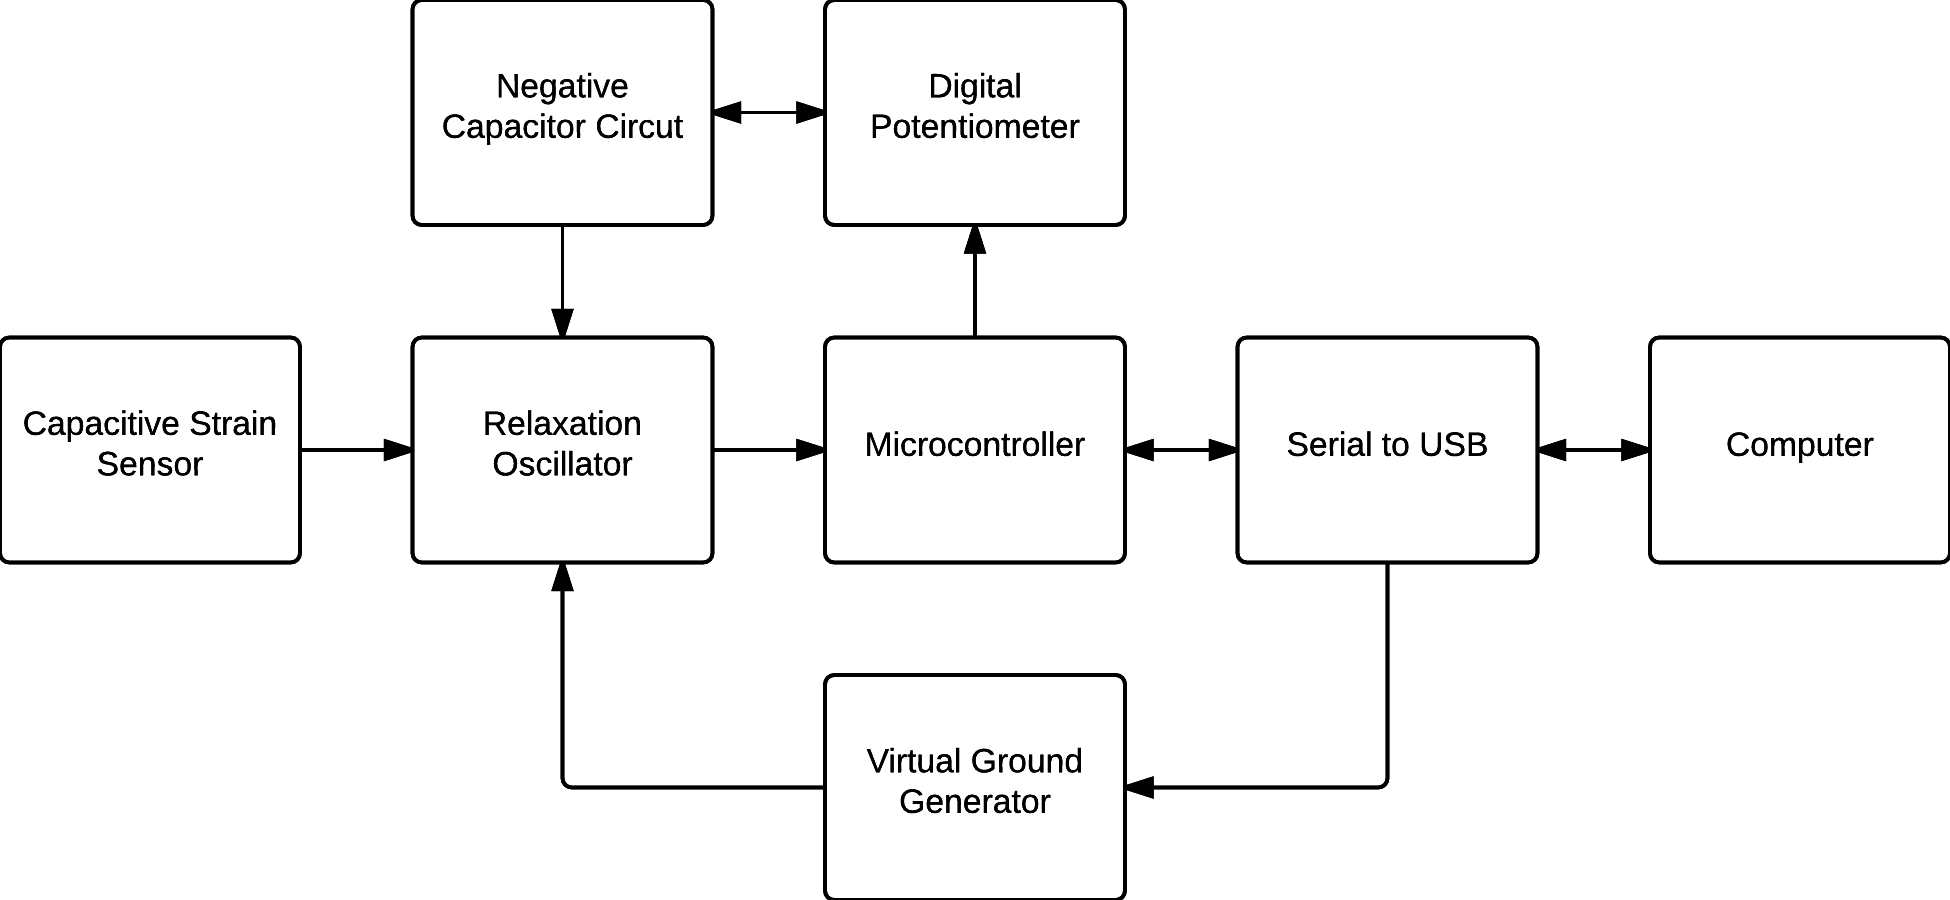
\includegraphics{Images/system-diagram.png}
		\caption{Data acquisition system diagram}\label{daq-system-fig}
	\end{center}
\end{figure}

\begin{figure}
	\begin{center}
		TODO: Need to change the passive values on the digital schematic and re-export since we re-tuned for the lower frequency.
		\caption{System schematic}\label{daq-schematic-fig}
	\end{center}
\end{figure}

\subsection{Measurement Method}
The measurement method is the aforementioned relaxation oscillator in conjunction with the negative capacitance circuit.  The capacitive strain sensor is connected directly to the relaxation oscillator circuit along with the negative capacitor circuit.  The potentiometer of negative capacitor circuit is provided by the digital potentiometer which is used for calibration of the system.  

The relaxation oscillator and negative capacitor circuits require positive and negative supply voltages to operate properly.  The system is powered from a single voltage source, and therefore these operational amplifier bias voltages must be created.  The system ground is chosen as the negative bias voltage and the system $V_{DD}$ is chosen as the positive bias voltage.  A virtual ground is created at the midpoint voltage between $V_{DD}$ and ground, and it is this virtual ground that is referenced for the analogue portions of the circuit.

%% mention the choice of R here

\subsection{Calibration}
The calibration is preformed using the digital potentiometer and the negative capacitor circuit.  The output frequency of the relaxation oscillator is selected by the parameters $C_{set}$, $R$, and the digital potentiometer set value.  The highest sensitivity for a given strain is achieved by selecting $R$ as large as physically possible and $C_{set}$ as close to the value of $C_0$ of the circuit as possible.  Therefore after these two values are set an unstrained frequency is selected to be as high as physically possible without degrading the physics of the capacitor to maximize sampling rate.  The value of the potentiometer is changed until the measured frequency matches the selected set point frequency.  

\subsection{Communication protocol}
The communication with the computer is over USB and connected as a virtual serial port.  The data transmitted from the data acquisition circuit to the computer is an ASCII formated string.  The format is ``\texttt{time, value\textbackslash n\textbackslash r}'' where \texttt{time} is a floating point time stamp in seconds and \texttt{value} is the raw measured value at that time.  The \texttt{\textbackslash n} is the linefeed character (ASCII 10) and \texttt{\textbackslash r} is the carriage return character (ASCII 13).  The value \texttt{time} starts at zero when the system is powered on and counts up at a resolution of 100 milliseconds.  The time stamp corresponds to the system time when the sampling process finished.  The \texttt{value} parameter is a raw value and can be converted into frequency using Equation \ref{daq-val-to-freq-eq} where $\beta$ is a scaling factor and is $32\text{MHz}$ on the current system.

\begin{equation}
	f_{sens}=\frac{\beta}{\texttt{value}}\label{daq-val-to-freq-eq}
\end{equation}

The strain of the sensor can be calculated from \texttt{value} as well.  Define the received raw value as $V$ and the set point raw value as $V_0$.  From Equations \ref{relax-eq5} and \ref{daq-val-to-freq-eq} Equation \ref{daq-val-to-cap} can be found.

\begin{eqnarray}
	f(\Delta C, k)=\frac{\beta}{V}&=&\frac{1}{2\ln(3)R(C_0+\frac{k-256}{k}C_{set}+\Delta C)}\\
	V&=&2\beta\ln(3)R\left(C_0+\frac{k-256}{k}C_{set}\right)+2\beta\ln(3)R\Delta C\\
	V&=&V_0+2\beta\ln(3)R\Delta C\\
	\Delta C&=&\frac{V-V_0}{2\beta\ln(3)R}\label{daq-val-to-cap}
\end{eqnarray}

% show how this relates to strain
\subsection{Microcontroller}
The microcontroller unit (MCU) selected for the data acquisition system was a PIC18LF2520.  This MCU was selected for its low power requirements, large amount of RAM, relatively high clock speed, and the well documented programming API.  The MCU also offered the peripherals needed for the system including input capture, serial peripheral interface (SPI), and universal asynchronous transceiver (UART).  

\subsubsection{Frequency Measurement}
The frequency of the capacitive strain sensor is measured using the input capture module of the MCU.  This module measures the time between events on a input pin.  The event used in this system was every sixteenth rising edge of the frequency signal.  By measuring the time between the first and sixteenth rising edge the average frequency of the signal over that time interval can be measured.

The time measurement of the current system is the system clock of 8MHz divided by four.  This gives a timer frequency of 2MHz or a minimum measurement resolution of 500ns.  ---PLACEHOLDER: add the calculation that this equates to 15fF resolution at 1kHz---.  An option is being currently explored to increase the system clock to 32MHz yeilding a time resolution of 125ns which greatly exceeds the 1fF requirement ---and this equation too---.   

The current system measures the average frequency averaged over sixteen pulses.  Assuming a nominal frequency of 1kHz this equates to a minimum of 16ms per sample and more when frequency is higher.  This is unable to meet the requirement of a 100Hz sample rate.   Options are being explored including changing the window from sixteen pulses down to eight pulses.  This would cut the per measurement sample time in half at the expense of also cutting the sensitivity in half.

\subsubsection{Calibration Potentiometer} 
The digital potentiometer used to calibrate the frequency communicates with the MCU over a serial peripheral interface (SPI).  The bus is used to serially set the position of the potentiometer.  It is also used to program the default potentiometer value into non-volatile memory inside the digital potentiometer.

\subsubsection{Communication}
Communication with the connected computer uses the universal asynchronous receiver and transmitter (UART).  The UART signal is connected to an FTDI UART to USB converter.  This converter connects to the computer and shows up as a virtual transport which can be written to and read from as if the circuit was plugged directly into the computers RS232 communications port.

\subsection{Software}
The software for the data acquisition system is relatively simple.  After a power-on-reset the MCU initializes the oscillator and other peripherals and then runs self calibration.  The self calibration sets the digital potentiometer to the midpoint value and measures the frequency.  It then increases or decreases as necessary and takes another frequency measurement.  This is repeated until the measured frequency matches the setpoint frequency within some tolerance.  The system then starts a system tick clock which interrupts every 250ms---Note to self: This will probably change to ever 100ms after dropping the samples down to 8 and getting the PLL to work---.  On each interrupt of this system clock a new frequency measurement is taken and that frequency along with the time it was taken is returned to the computer over the UART to USB connection.  This process is repeated indefinitely until the user stops it.  

The system receives commands over the UART. Commands are delimited by line feed characters (ASCII 10) at which time the command is deciphered asynchronously in an interrupt routine.  Currently three types of commands are supported.  The first command is a number between 0 and 255 inclusive.  This command is used as a new digital potentiometer value and applied immediately.  The second command is an ASCII `c' character followed by a number.  The number following the `c' is used as a new frequency set point value and the system is immediately recalibrate to that new frequency.  The frequency is as a raw value which corresponds to a real frequency using Equation \ref{daq-val-to-freq-eq}.  The final command currently supported is the ASCII character `r' which causes the system to do a hard reset.  This will recalibrate the frequency to its power on default and restart the time stamp count at zero.


